\chapter{Solving Recurrences}

\section{The Master Theorem}

If $T(n) = aT(\frac{n}{b}) + O(n^d)$, then

\begin{math}
T(n) = \left\{
\begin{array}{l l}
O(n^d)       & \quad \text{if} d > log_ba \\
O(n^d logn)  & \quad \text{if} d = log_ba \\
O(n^{log_ba}) & \quad \text{if} d < log_ba \\
\end{array} \right.
\end{math}

\section{Recursion Tree}

We can reason about a recurrence of the form: $ T(n) = aT(\frac{n}{b})
+ f(n) $ where $ a \geq 0, b > 0 $ with the following recursion tree:

{
  % Current graphic is hand-drawn by John Howat.
  % Should replace asap with a nicer diagram
  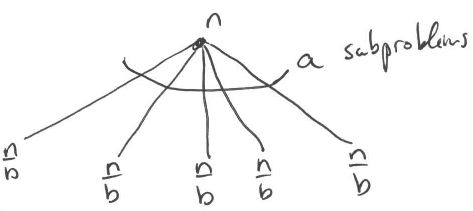
\includegraphics[scale=1.2]{recursion_tree}
  %\caption{A recursion tree representing a recursions on n/b elements}
  \label{fig:recursion_tree}
}

This tree has the following properties:

\begin{enumerate}
\item The number of nodes at level $i$: $a^i$
\item Work done at each node of level $i$: $f(\frac{n}{b^i})$
\item Number of levels: $log_bn$
\item Number of leaves: $n^{log_ba}$
\end{enumerate}

We can use this information to solve the recurrence:

\begin{align*}
T(n)
&= \sum\limits_{i=0}^{log_bn} 
(\text{\# nodes at level } i) 
(\text{work done at level } i) \\
&= \sum\limits_{i=0}^{log_bn} a^i f(\frac{n}{b^i})
\end{align*}
